\chapter{Teams and Teamwork}
\graphicspath{ {./chapter09/Fig} }

\begin{itquote}
The way a team plays as a whole determines its success. You may have the
greatest bunch of individual stars in the world, but if they don't play
together, the club won't be worth a dime.---Babe Ruth
\end{itquote}

Engineering projects are often very large and require too many diverse
skills to be completed by a single person. This necessitates the use of
teams, and it is likely that you will participate on many during your
professional career. That is why employers of engineering graduates
consistently rate teamwork ability as one of the most desirable
attributes in a potential employee. Teams can collectively perform tasks
that could not possibly be completed by individuals working in
isolation. However, just because a team is created does not mean that it
will function effectively, and examples of failed teams abound. When
people learn that they are going to work on a team, their initial
reaction is often one of dread, usually due to bad experiences in the
past. The good news is that with some attention to team principles and a
conscious effort, working on a team can be a positive experience. Much
research has been done and much has been written on teams and teamwork.
The objective of this chapter is to provide a primer on what constitutes
a team, present models of team development, identify the characteristics
of effective teams, and provide guidance for effective teamwork.

\section*{Learning Objectives}
\noindent\rule{\linewidth}{1pt}
By the end of this chapter, the reader should:

\begin{itemize}
\item
  Understand the characteristics that define a team and understand why a
  team is formed.
\item
  Understand different models for the stages of team development.
\item
  Understand the characteristics of effective teams.
\item
  Be able to develop Team Process Guidelines.
\end{itemize}

\section{What is a Team?}
\label{section:what-is-a-team}

The concept of a team is used broadly in many different contexts, so the
following definition of a team proposed by Katzenbach and Smith in
\ul{The Wisdom of Teams} {[}Kat93{]} is provided for the basis of our
discussion:

\begin{itquote}
A small group of people with complementary skills, who are committed to
a common performance, performance goals, and approach for which they
hold themselves mutually accountable.
\end{itquote}

This concept of a team is highly relevant to engineering design
projects.

The definition indicates that a team should be a small group of people,
typically two to ten. Teams larger than this become very difficult to
manage. The reason is that the number of relationships between people
increases rapidly with an increase in the number of people on the team.
The number of person-to-person relationships is equal to
$n(n-1)/2$ is number of people on the team. Any one
of these relationships can falter, causing problems. In addition, it is
hard to develop consensus on important issues as the number of people on
the team increases.

Second, the definition indicates that teams should be composed of
members who have complementary skills. Members should be selected based
upon the background and skills that each person brings to the team, not
based upon personality and friendships. This leads to the related
concepts of \emph{\textbf{cross-functional}} and
\emph{\textbf{multi-disciplinary teams.}} Cross-functional teams are
those that are composed of people from different organizational
functions, such as engineering, marketing, and manufacturing
{[}Wil95{]}. Cross-functional teams are particularly important in new
product development, where multiple functions are required to bring a
product from concept, to manufacture, and ultimately to the market.
Multi-disciplinary implies that the team is composed of members from
different disciplines. There is no agreement in the engineering
community as to what exactly constitutes a multi-disciplinary team. In
general, the idea of complementary skills applies where a team may have
representation from multiple technical disciplines. For example, the
development of a robot would require members with multi-disciplinary
expertise in computing, electronics, and mechanical systems.

Third, the definition states that teams should have common performance
goals. The goals take time to develop and the team will likely flounder
in creating them, but without specific goals to achieve there is no need
for a team. In the context of design, the team's goals are defined by
the Problem Statement and Requirements Specification developed in
Chapters 2 and 3 respectively. They collectively state what the team is
trying to achieve and provide a way for the team to verify its
success---are the requirements met and can the team demonstrate that
they are?

Finally, the team definition indicates that teams should have a common
approach for which they hold themselves mutually accountable. This can
be a common approach to solving problems, such as application of the
design process. It can also be in terms of a method for holding the team
members accountable. One of the biggest problems that teams face is
handling situations where the team fails to meet a given objective. This
may be due to one or more members failing to meet their commitments. The
team must be able hold each other mutually accountable in a constructive
manner in these situations.

\section{Models of Team Development}
\label{section:models-of-team-development}

Bruce Tuckman developed a model for team development that contains fives
stages, known as forming, storming, norming, performing, and adjourning
{[}Tuc65{]}. It is instructive to have an understanding of these stages
so that you are aware of the dynamics that occur as a team develops. The
five stages are described as follows:

\begin{itemize}
\item
  \emph{Forming.} This is the stage where the team is created. The team
  members may not know each other, leading them to be anxious and
  uncomfortable. It is likely that the team's objectives are not
  well-defined and that the members' roles are ambiguous.
\item
  \emph{Storming.} In this stage, the team works to develop its
  objectives, while the members try to define their roles. Conflict
  often appears as members jockey for position and advantage. It is
  characterized by fighting and power struggles, which may be overt, but
  in many cases are subtle and below the surface. The team must resolve
  individual versus group goals. For example, what if the team is trying
  to select a project concept? Some members may have strong opinions and
  preconceived notions about what the project should be. Failure to
  navigate the storming stage means that the team will not reach the
  performing stage and will be forced to return to the storming stage at
  some time.
\item
  \emph{Norming.} In this stage the team starts to become more cohesive.
  Members accept the team's objectives, their roles on the team, and
  they agree upon procedures. In this phase the team develops common
  approaches for solving problems and managing conflicts.
\item
  \emph{Performing.} In this stage, the team focuses on performing tasks
  and achieving the objectives set forth. The team should be
  collaborating and easily making decisions. Disagreements that arise
  are accepted and resolved by the team norms.
\item
  \emph{Adjourning.} Here, the team dissolves, hopefully due to
  successful project completion. However, it can occur abruptly if the
  project is cancelled, or even worse, if the team is unable to function
  together.
\end{itemize}

Katzenbach and Smith proposed the team performance curve in 
Figure~\ref{figure:teamPerformance},
which shows the performance impact of teams versus varying levels of
effectiveness. The types of teams they defined are the working group,
the pseudo-team, the potential team, and the high-performance team. The
most closely related stages of team development from the Tuckman model
are indicated in parentheses on the figure. Notice that the scale on the
x-axis is team effectiveness, not time. There may be an implicit
assumption that teams will move through these stages as a function of
the time the team is together. That is certainly a desired goal, but not
necessarily what the model implies.

\begin{figure}
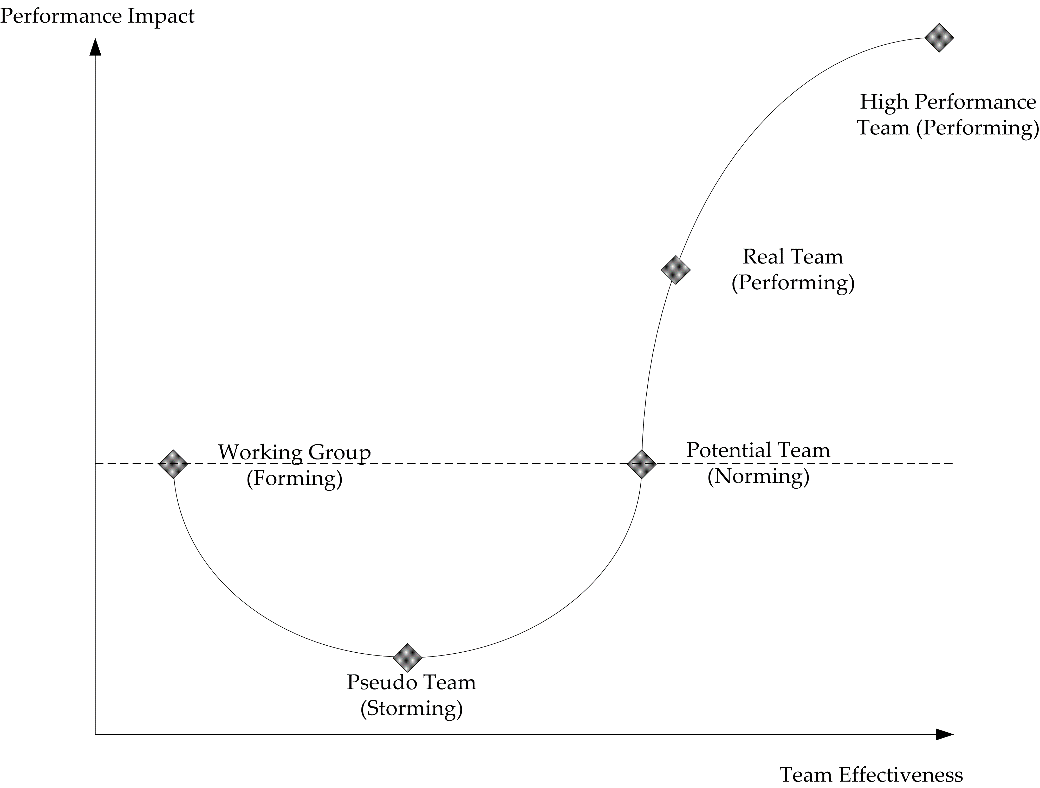
\includegraphics[width=4.73in,height=3.59in]{./image1.png}
\caption{The team performance curve proposed by Katzenbach
and Smith {[}Kat93{]}. This shows the performance impact of teams versus
varying levels of effectiveness. The Tuckman stages of team development
(forming, storming, norming, performing) that are most closely related
to the performance points are superimposed on the model {[}Tuc65{]}.}
\label{figure:teamPerformance}
\end{figure}

The \emph{\textbf{working group}} is defined as a group of individuals
working in isolation, who come together occasionally to share
information. In other words, if every member of the team works in
isolation and meets only to share ideas, they would achieve the
performance of the working group. This level of performance is
represented by the dashed baseline. In fact, the working group is not a
team as given by the definition and serves a very different purpose. The
\emph{\textbf{pseudo-team}} represents an under-performing team where
the sum effort of the team is below that of the baseline performance,
while the \emph{\textbf{potential team}} is one in which the team is
functioning at a level equal to that of the working group. At a minimum,
teams should at some point perform above the level of a potential team,
otherwise, there is no need for a team. The objective is to perform at
the level of a \emph{\textbf{real team,}} where the performance exceeds
that of the working group. In rare instances the level of a
\emph{\textbf{high-performance team}} may be realized in which the team
significantly outperforms all similar teams.

\section{Characteristics of Real Teams}
\label{setion:characteristics-of-real-teams}

How can a team reach the performing stage and simultaneously become a
real team? Unfortunately, there is no set process for guaranteeing that
a team will become a real team. There are characteristics and principles
of effective teams, and it has been observed that real teams apply these
principles. However, realize that there is a difference between a team
and teamwork principles. Real teams apply teamwork principles but this
does not imply that the converse statement is true---that applying these
principles will result in a real team. The lesson is that successful
teams adhere to good teamwork principles, but the application of good
teamwork principles does not automatically guarantee that teams will be
successful. However, ignoring teamwork principles almost always leads to
failure. The remainder of this section presents some of the
characteristics of real teams.

\subsection{Select Members Based Upon Skills}
\label{subsetion:select-members-based-upon-skills}

Selecting team members based upon their skills is a key to success
identified by Katzenbach and Smith. They defined three categories of
relevant skills: 1) technical and functional, 2) problem-solving, and 3)
interpersonal. The right mix of technical skills on a design project is
important to achieve the desired objectives, reinforcing the need for
multi-disciplinary and cross-functional teams. Different problem-solving
approaches and the mix of interpersonal skills are important as well,
but harder to determine. The Meyers-Briggs personality tests or the
Keirsey Temperament sorter {[}Kei84{]} are tools that can be used to
identify different problem-solving approaches and personality traits,
but in themselves are not the answer for selecting teams.

One important point to consider is whether teams should be formed by
self-selection or assigned by a supervisor. There are pro and con
arguments for each method of selection. An argument for self-selection
is that members believe the objectives of the team are important,
leading to a higher level of commitment. A potential pitfall is that not
enough attention is paid to the skills necessary to complete the
project. In the second case, teams are assigned by someone who has an
understanding of the skills needed for the project and assigns members
accordingly. A potential pitfall is that this may create animosity from
team members who are dissatisfied with the project from the outset.

\subsection{Identify Objectives}
\label{subsection:identify-objectives}

Teams are created to realize shared goals, and if the goals are not
well-defined, the motivation for being part of the team is not clear. In
the context of engineering design, the combined Problem Statement and
Requirements Specification presented in Chapters 2 and 3 serve that
purpose. The Problem Statement describes what the team is trying to
achieve, while the Requirements Specification sets verifiable targets
that define success. Both items are so important, that there should be a
consensus agreement among the team members on their content. The team
should be challenged by targets that are aggressive, yet achievable.
Identifying measurable objectives was identified by Katzenbach and Smith
as one of the most important attributes of successful teams. Further,
all team members must be committed to achieving the objectives.

\subsection{Develop Decision-Making Guidelines}
\label{subsection:develop-decision-making-guidelines}

Teams regularly make decisions that affect all of its members and the
success of the project. The team must determine how decisions are to be
made, and once they are, all members need to accept the outcome. The
team also needs to understand the importance of different
decisions---not all are equally important and different approaches
should be used depending upon the impact of the decision. Models for
decision-making are outlined as follows {[}Joh02{]}:

\begin{enumerate}
\def\labelenumi{\arabic{enumi}.}
\item
  \emph{Decision by Authority}. The leader makes all decisions,
  typically without discussion by the rest of the team. This is
  effective for fast decision-making, but does often not lead to the
  best decision. It can also produce resentment among the team.
\item
  \emph{Expert Member}. The most expert member on the subject decides.
  This is effective in cases where there is a single member who is
  clearly the expert on the subject.
\item
  \emph{Average Member Opinion.} The average team member opinion is
  used. A method needs to be devised to determine what constitutes the
  average opinion.
\item
  \emph{Decision by Authority after Discussion.} The leader makes a
  decision after all team members discuss the issue and provide input.
\item
  \emph{Minority Control.} A few members act as a subcommittee and solve
  the problem. This makes sense if the minority group consists of
  experts on the particular problem.
\item
  \emph{Majority Control.} A simple majority is used to make decisions.
\item
  \emph{Consensus.} All team members must agree to and commit to the
  decision. This generally comes after much discussion and evaluation of
  the different alternatives. This is the best approach, and the most
  time-consuming. It is not necessary for all decisions to be made this
  way, but consensus should be reached for important decisions.
\end{enumerate}

A formal and widely used method for brainstorming and team
decision-making is known as the \emph{\textbf{Nominal Group Technique}}
(NGT) {[}Del71{]}. NGT was covered in Chapter 4 and is repeated here. In
NGT, each team member silently generates solutions to a problem and the
ideas are then reported out in a round-robin fashion until all ideas are
exhausted. Then, each member gets to cast a predetermined number of
votes for the ideas presented. The top idea is then selected, or
alternatively, the top few ideas are discussed further and voted upon
again. The steps of NGT are outlined below:

\begin{enumerate}
\def\labelenumi{\arabic{enumi}.}
\item
  \emph{Read problem statement.} It should be read out loud by a team
  member (the facilitator).
\item
  \emph{Restate the problem.} Each person restates the problem in their
  own words to ensure that all members understand it.
\item
  \emph{Silently generate ideas}. All members silently generate ideas
  during a set period of time, typically 5­--15 minutes.
\item
  \emph{Collect ideas in a round-robin fashion}. Each person presents
  one idea in turn until all ideas are exhausted. The facilitator should
  clarify ideas and all should be written where the entire team can view
  them.
\item
  \emph{Summarize and rephrase ideas.} Once the ideas are collected, the
  facilitator leads a discus­sion to clarify and rephrase the ideas. This
  ensures that the entire group is familiar with them. Related ideas can
  be grouped or merged together.
\item
  \emph{Vote.} Each person casts a predetermined number of votes,
  typically three to six, for the ideas presented. The outcome is a set
  of prioritized ideas that the team can further discuss and pursue.
\end{enumerate}

\subsection{Hold Effective Meetings}
\label{subsection:hold-effective-meetings}

Teams need to meet for a variety of reasons, such as determining
objectives, tracking progress, assigning tasks, preparing deliverables,
and resolving problems. It is in these meetings that teamwork principles
are most critical and where problems can arise. In the workplace it is
estimated that people spend half of their time in tasks that are related
to meetings (preparing, attending, and following up). Three elements of
effective meetings are: 1) well-defined roles for the participants, 2) a
structure for conducting the meeting, and 3) the application of
interpersonal skills {[}Bel94{]}. Poorly organized and ineffective
meetings lead to cynicism and poor team performance. The structure of
meetings does not always need to be the same. Some keys to effective
meetings are:

\begin{itemize}
\item
  \emph{Have an agenda.} Agree upon the goals for a meeting in advance.
\item
  \emph{Show up prepared.} All members should show up on time with their
  tasks completed.
\item
  \emph{Pay attention.} Each person should speak in turn, and there
  should be no disruptive side conversations. No person should
  monopolize the conversation and all points of view should be heard.
\item
  \emph{Agree upon a meeting time and place.} People have busy schedules
  and different work habits. Believe it or not, failure to agree upon
  this basic issue can lead to tremendous conflict.
\item
  \emph{Summarize.} At the end of the meeting summarize what was
  discussed, important decisions made, and actions to be taken.
\end{itemize}

\subsection{Develop Team Roles}
\label{subsection:develop-team-roles}

As the group finds its norms, members should settle into different
roles. They may be based upon the technical aspects of the design, such
as hardware, software, and mechanical systems. The team may find that
certain members are more effective at different tasks such as procuring
parts, making presentations, and writing technical documents. Roles
often evolve and change as the team develops.

Team roles are usually not known early on in the forming stage and
members can be assigned formal roles to perform in at the outset. This
is also common in group problem solving sessions and a typical set of
roles follows {[}App01{]}:

\begin{itemize}
\item
  \emph{Leader.} The leader is not necessarily the authority figure, but
  should guide the team through the processes of decision-making and
  problem-solving. Effective leaders should ensure that all opinions are
  heard and that everyone is involved. Leaders coordinate tasks such as
  identifying the agenda.
\item
  \emph{Recorder.} The recorder is responsible for maintaining a record
  of the team's work, documenting important results, and recording
  responsibilities for different tasks.
\item
  \emph{Spokesperson.} The spokesperson articulates the team's results.
  The recorder and spokesperson roles are sometimes combined.
\item
  \emph{Optimist.} The optimist's role is to examine reasons why ideas
  and concepts will work, find their merit, and advocate other's ideas.
\item
  \emph{Pessimist.} The pessimist should challenge ideas and
  assumptions, and make sure that opposing ideas are presented and
  discussed.
\item
  \emph{Analyst.} The team analyst performs the important role of
  observing the team processes and provides feedback to the team for
  improvement.
\end{itemize}

The roles presented here are by no means definitive and other models
having different roles can be utilized. The common thread is to have
participants gain experience in the different roles so that they can
become more effective team members. No matter what role a member is
playing, they should all contribute to the solution of the problem at
hand. As the team evolves and becomes more experienced, the need for
formal roles will diminish.

\subsection{Assign Tasks and Responsibilities}
\label{subsection:assign-tasks-and-responsibilities}

Nothing creates problems more than when team members do not have clearly
defined responsibilities and tasks. The workload needs to be distributed
in a fair manner and all members must perform real work. Without this,
one or two people do most of the work, or even worse, nothing gets done.
Chapter 10 presents project management principles, one of the primary
aims of which is to develop and assign tasks to team members. Teams may
consider designating one person as the project manager who is
responsible for tracking the team's progress and ensuring that members
are meeting their commitments. It is important that the project manager
also be assigned tasks, outside of project management, that contribute
to the project.

\subsection{Spend a Lot of Time Together}
\label{subsection:spend-a-lot-of-time-together}

Teams that spend a lot of time together are generally more successful
{[}Kat93{]}. This is not only time together in meetings and working on
project deliverables, but also includes extracurricular activities. All
members of the team should be included, not just a subgroup. Experience
shows that on teams of three students, two members may spend a great
deal of time together and form a bond. This can alienate the third
person (not necessarily intentional) and lead to conflict.

\subsection{Respect Each Other}
\label{subsection:respect-each-other}

Imagine a scenario where you are assigned to a team and one of the
members is that quiet, weird guy who never says anything, or that
loudmouth who never shuts up. You may have a real challenge ahead of
you, but working with people who are not our best friends is a reality
of life. You have to learn how to deal with personality issues if you
want to be effective on teams. One key is to demonstrate respect for the
other members of your team. Ways to do this are to:

\begin{itemize}
\item
  \emph{Listen actively.} Most people are not effective listeners. As
  they listen to others they are mentally formulating their response,
  while not actually listening to the other person. By listening to the
  other person, then formulating an appropriate response, you will
  develop a better understanding of their viewpoint and demonstrate that
  their opinion is being heard.
\item
  \emph{Consider how you respond to others.} How you respond to others
  impacts your effectiveness. Are you negatively evaluating others ideas
  or treating their ideas unfairly?
\item
  \emph{Constructively criticize ideas, not people.} It is fine to
  examine problems and constructively criticize ideas. Consider looking
  for ways to improve upon ideas that have flaws.
\item
  \emph{Respect those not present.} Nothing creates divisions and
  factions in a team faster than personally criticizing members not
  present. If a team member is not performing, refer to the Team Process
  Guidelines examined in Section 9.4 for holding them accountable.
\item
  \emph{Communicate your ideas.} If you have an idea, clearly state it
  and be prepared to explain what the merits are. Be prepared for
  critical analysis and discussion of the idea.
\end{itemize}

\subsection{Manage Conflicts Constructively}
\label{subsection:manage-conflicts-constructively}

Conflicts inevitably occur on teams, and the more constructively they
are addressed the better. Real teams do encounter conflicts, but they
are adept at resolving them. Conflicts can be good, particularly when
they lead the team to the solution of a problem or the development of
consensus. They also provide an opportunity for members to express their
opinions on important issues. Left unresolved and unspoken, they lead to
resentment, suspiciousness, and escalate into personal conflicts.
Conflicts may be false (you misinterpret another's behavior), based on
performance (member(s) aren't doing their work, or it is of poor
quality), or based upon procedure (disagree with the way that meetings
are run or decisions are made) {[}Dom01{]}. Some strategies for
resolving conflicts are:

\begin{itemize}
\item
  \emph{Focus on performance and ideas.} Focus on the performance of the
  team and not individual personality. Also, focus on ideas and
  constructively criticize them.
\item
  \emph{Listen to others.} It is very important to remain calm and
  listen carefully to others when conflicts arise.
\item
  \emph{Identify concerns.} If you have concerns about something, it is
  best to identify and address them, rather than hiding them.
\item
  \emph{Apply the team's process guidelines.} In the next section, a
  format for process guidelines that govern the behavior and processes
  of a team is given. This should address a team's approach for
  resolving conflicts. Importantly, the team must remember to apply the
  guidelines when conflicts arise.
\item
  \emph{Develop a plan to resolve the conflict.} Again, conflict can be
  positive and lead to the solution of problems. The team may not be
  able to resolve a conflict immediately, but can develop a plan for
  solving it within a specified period of time.
\item
  \emph{Mediation.} A mediator can be used after all avenues for
  resolution of the conflict have been exhausted. One way to do this is
  to employ a variation of the Delphi Technique. The Delphi Technique
  was originally developed as a brainstorming method to generate ideas
  anonymously from experts outside of a team or organization. It is
  applied for mediation through the following steps:
\end{itemize}

\begin{enumerate}
\def\labelenumi{\arabic{enumi}.}
\item
  Each member of the team should anonymously supply a description of the
  conflict and suggested remedies to the mediator.
\item
  The mediator proposes a solution to the conflict, which is fed back to
  the team.
\item
  The team members are given an opportunity to suggest modifications to
  the proposed resolution.
\item
  Steps 1-3 are repeated until consensus is achieved.
\end{enumerate}

\section{Project Application: Team Process Guidelines}
\label{section:project-application-team-process-guidelines}

Teams should develop clear and detailed guidelines that govern their
processes. These guidelines are based on the items covered in the
previous section. The entire collection of guidelines forms the
\emph{\textbf{Team Process Guidelines}}. Issues addressed in the Team
Process Guidelines include:

\begin{itemize}
\item
  \emph{The team's name.} This creates an early opportunity for
  decision-making.
\item
  \emph{The team's mission and objectives.} This can be a brief
  re-statement of the design problem statement.
\item
  \emph{Decision-making guidelines.} Indicate what techniques are going
  to be used to make decisions and when they will be applied.
\item
  \emph{Meeting guidelines.} How will meetings be run and what are the
  expectations for team members in the meetings.
\item
  \emph{Team roles.} If teams self-select, they should justify their
  team choice with identification of the complementary skills each
  member brings to the team.
\item
  \emph{Conflict resolution.} Identify how the team will resolve
  conflicts. For example, what will the team do when members are doing
  sub-standard work and not meeting the performance objectives? How will
  the team determine what sub-standard performance is? What happens if a
  member misses a meeting? What will the team do if they cannot resolve
  the conflict among themselves?
\end{itemize}

This document should be developed early on, referred to regularly
throughout the project, and updated by the team as necessary. Table 9.1
contains a checklist and self-assessment of the team formation stage and
processes.

\section{Summary and Further Reading}
\label{section:summary-and-further-reading}

This chapter touched on some of the fundamental concepts of team
development that have been reported in the literature. Two well-known
models of team development were presented. The first is the Tuckman
model of the forming, storming, norming, performing, and adjourning
stages. It is important for teams to carefully navigate the formative
stages, agree upon the objectives, and reach the performing stage. The
second is the Katzenbach and Smith team performance curve presented in
Figure 9.1. Selected characteristics of real teams were identified.
Finally, Team Process Guidelines are a tool for identifying a team's
norms, problem solving approach, and self governing principles. A format
for the guidelines was presented.

There are many excellent books and resources available that examine
teams and teamwork. One that influenced this chapter greatly is \ul{The
Wisdom of Teams} by Katzenbach and Smith {[}Kat93{]}. It is a seminal
work in the field and a widely recognized resource that addresses how to
create effective teams. The forming, storming, norming, performing, and
adjourning model of team development was proposed by Bruce Tuckman
{[}Tuc65{]} and is widely documented as a good model for team
development. \ul{The Team Training Workbook} {[}Bel94{]} is another
valuable resource developed by Arizona State University engineering
faculty members. \ul{Teamwork and Project Management} by Karl Smith
{[}Smi04{]} is a short introduction to both teamwork principles and
project management for engineering students. Free personality tests and
temperament sorters can be found online; one example being the Keirsey
Temperament Sorter at
\href{http://www.advisorteam.com/}{www.advisorteam.com}.


\begin{table}
\caption{Checklist and self-assessment for team formation and
processes. 1 = Strongly Disagree, 2 = Disagree, 3 = Neutral, 4= Agree, 5
= Strongly Agree.}
\label{table:teamCheckList}
\begin{tabular}{|m{15cm}|l|}
\hline
\rowcolor{Gray}
\textbf{Team Formation} & \textbf{Score} \\ \hline
The team's objectives are clearly defined. & \\ \hline
There is consensus among all team members that the objectives are the
correct ones. & \\ \hline
The team members complementary skills (technical, functional,
interpersonal) have been identified. & \\ \hline
There are enough members on the team to cover all of the necessary
competencies. & \\ \hline
There are not too many members on the team. & \\ \hline
\rowcolor{Gray}
\textbf{Team Processes} & \\ \hline
The team has developed clear guidelines for resolving conflicts and
disagreements. & \\ \hline
The team has developed effective guidelines for holding all members of
the team mutually accountable for achieving the objectives. & \\ \hline
The team has developed a strategy for holding effective meetings. & \\ \hline
The team has agreed upon a mutual meeting time and place. & \\ \hline
The team members trust each other. & \\ \hline
The team members demonstrate respect for each others ideas. & \\ \hline
\end{tabular}
\end{table}
